\documentclass[a4paper,12pt]{article}
\usepackage[utf8]{inputenc}
\usepackage[french]{babel}
\usepackage[T1]{fontenc}
\usepackage{graphicx}
\usepackage{pgf}
\usepackage{geometry}
\geometry{hmargin=2cm,vmargin=2cm}
\usepackage{caption}
\usepackage{subcaption}
\usepackage{fancyhdr}
\usepackage{hyperref}
\usepackage{multicol}
\usepackage{amsmath, amssymb}
\usepackage{mathrsfs}
\usepackage{calrsfs}\usepackage{cases}
\usepackage{vmargin}
\usepackage{graphicx}
\pagestyle{fancy}
\usepackage{listings}
\lstset{upquote=true, columns=flexible, basicstyle=\ttfamily\bfseries, captionpos=b}

\usepackage[normalem]{ulem}

\newenvironment{mld}
{\par\begin{minipage}{\linewidth}\begin{tabular}{rp{0.7\linewidth}}}
{\end{tabular}\end{minipage}\par}
\newcommand{\relat}[1]{\textsc{#1}}
\newcommand{\attr}[1]{\emph{#1}}
\newcommand{\prim}[1]{\uline{#1}}
\newcommand{\foreign}[1]{\#\textsl{#1}}

%%%% options %%%%%
\headwidth = \textwidth
\title{Projet SGBD}
\renewcommand{\headrulewidth}{1pt}
\fancyhead[L]{\textsc{Projet de Base de Données}}
\fancyhead[R]{page {\thepage}}

\renewcommand{\footrulewidth}{1pt}
\fancyfoot[R]{} 
\fancyfoot[L]{\small{\leftmark}}
\fancyfoot[C]{}

\newcommand{\xmark}{\sffamily X}


\begin{document}
\begin{titlepage}
\thispagestyle{empty}
\vspace{\stretch{1}}
\begin{sffamily}
  \begin{center}
  \textsc{\LARGE Enseirb-Matmeca}\\[2cm]
  \textsc{\LARGE Informatique 2$^e$ année}\\[2cm]
  \end{center}
  \end{sffamily}
  
\noindent \rule{\textwidth}{0.5pt}
  \begin{center}
  \Huge
  \textbf{Fédération Sportive de Basket-ball}
  \end{center}
\noindent \rule{\textwidth}{0.5pt}

\begin{center}
\textbf{Auteurs : Simon Dellac, Guillaume Douezan-Grard\\ Julien Marzin}
\end{center}
\vspace{2cm}
\begin{center}

\includegraphics[scale=1.1]{logo.png}
\end{center}
\vspace{2cm}

\begin{center}
Date : 12 Décembre 2014
\end{center}

\vspace{\stretch{1}}
\end{titlepage}

\tableofcontents
\clearpage

\section*{Introduction}
\addcontentsline{toc}{part}{Introduction}
L'objectif de ce projet est de réaliser une base de données gérant les rencontres de Basket-Ball entre les différents clubs d'une fédération. Un club est constitué de plusieurs entités telles que:
\begin{itemize}
\item un bureau ;
\item des équipes ;
\item des joueurs ;
\item des entraineurs ;
\item des catégories.
\end{itemize}
\vspace{0.25cm}
Les clubs de la fédération réalisent des rencontres à une certaine date. On veut pouvoir stocker les statistiques des joueurs participant à ces rencontres. Notre base de données doit donc stocker toutes ces informations. Elle doit également pouvoir être consultée, mise à jour ou détruite.

Afin de créer la base de données réalisant cette fédération, nous avons élaboré plusieurs diagrammes Entité-Association.

\section{Modélisation des données}
Dans cette partie, nous présentons les diagrammes que nous avons réalisés lors de l'élaboration de notre base. Nous commençons par notre diagramme entité-association initial, puis nous exposons le modèle entité-association retenu.

\subsection{Diagramme Entité-Association}
\subsubsection{Modèle initial}
Nous avons commencé par vouloir regrouper un maximum d'informations dans différentes tables. Vous trouverez en figure \ref{EAinit} le premier modèle que nous avions élaboré.\\

Les problèmes principaux étaient les nombreuses contraintes d'intégrité fonctionnelle entre les différentes entités du modèle. Par exemple, un joueur ne pouvait pas être un entraîneur et inversement. D'autre part, nous stockions le nombre de matchs gagnés, perdus et nuls dans l'entité équipe. Ces informations étaient redondantes, car il est possible de les retrouver  en utilisant les attributs «score» de l'entité rencontre. Sur ce premier modèle, nous avions également une unique équipe reliée à l'entité rencontre. Cela pose problème, car deux équipes exactement doivent participer à une rencontre. Il aurait fallu ajouter une clef étrangère aux équipes pour retrouver une rencontre. Mais dans ce cas, il fallait aussi vérifier que deux équipes exactement possédaient une même clef étrangère.

Dans ce diagramme, l'entité catégorie était peu utile, en effet chaque équipé ayant un identifiant unique, il est possible de stocker le nom de catégorie dans l'entité équipe. Il n'y pas de problème pour un club à avoir plusieurs équipes dans une même catégorie.\\


\begin{figure}[!h]
\centering
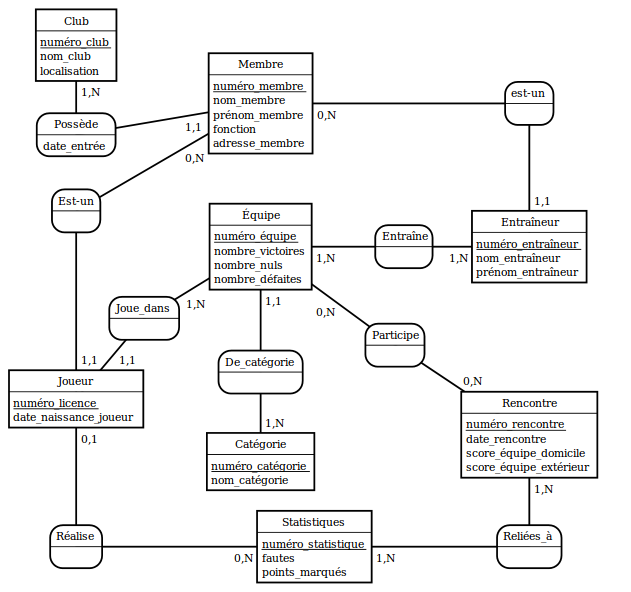
\includegraphics[scale=0.6]{init.png}
\caption{Modèle Entité-Association initial\label{EAinit}}
\end{figure}

En raison de ces contraintes, nous avons cherché à obtenir un modèle plus ergonomique.
\subsubsection{Modèle retenu}
Le modèle retenu est présenté en figure \ref{EAretenu}. Les principaux changements ont été de déplacer certains attributs et de séparer les membres d'un club qui sont membres du bureau et ceux qui sont entraineurs et/ou joueurs. (Les membres du bureau peuvent également être joueurs et/ou entraîneurs).

\begin{figure}[!h]
\begin{minipage}{.96\linewidth}
\centering
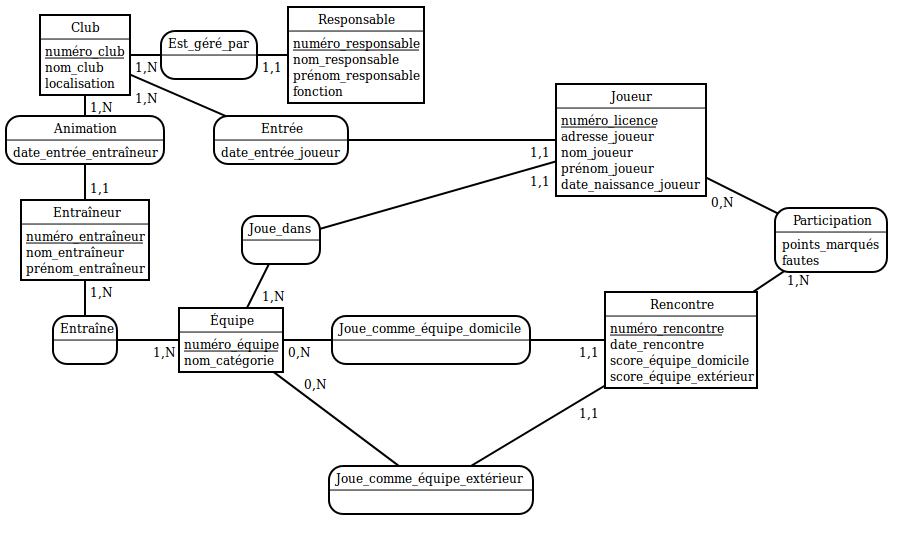
\includegraphics[scale=0.6]{modeleea.png}
\caption{Modèle Entité-Association retenu\label{EAretenu}}
\end{minipage}
\end{figure}

Les \textbf{hypothèses} que nous avons faites sont les suivantes :
\begin{itemize}
\item chaque responsable d'un club exerce une et une seule fonction. Par exemple, le président d'un club ne peut pas être trésorier ce club.
\item A priori, un entraîneur ne peut pas être un joueur. On peut cependant avoir un joueur-entraîneur dans un club. Le défaut est que son nom, son prénom et sa date d'entrée sont présents en double dans la base. Cette situation étant très rare, nous n'avons pas souhaité faire de modification sur ce point.
\item Une rencontre se fait entre deux équipes qui sont de même catégorie.
\item Les joueurs d'une équipe peuvent ne pas participer à une rencontre, ils ne possèdent alors pas de statistiques.
\item Un entraineur peut entraîner une ou plusieurs équipes mais dans un seul club.
\end{itemize}
\vspace{0.2cm}
Les autres choix que nous avons fait concernent les attributs de certaines entités.\\

En ce qui concerne les \emph{rencontres}, nous avons décidé de les lier à deux équipes. Nous avons choisi de stocker le score de chacune des équipes dans cette entité, car cela permet de simplifier certaines requêtes de statistiques. Par exemple, sans ces attributs pour vérifier la victoire d'une équipe, il faudrait additionner les points marqués par chaque joueur de l'équipe lors de la rencontre donnée. Pour compter plusieurs victoires, cela devient rapidement compliqué. Nous avons aussi ajouté un attribut journée dans les rencontres. Une journée (chiffre) définit une plage de date où un ensemble de rencontres est joué dans le championnat par plusieurs équipes. Cet attribut nous semble pertinent pour réaliser des requêtes sur plusieurs rencontres. Par exemple en cas de rencontre reportée, on peut tout de même prendre en compte dans le classement le résultat des équipes pour la journée de cette rencontre. \\

Pour les \emph{catégories}, nous avons décidé de les stocker dans l'entité équipe. En effet, chaque équipe ayant un identifiant unique, il est possible de stocker la catégorie dans cette équipe. Plusieurs équipes dans un même club peuvent être dans la même catégorie sans problème.\\

Les tables \emph{animation} et \emph{entree} ont été créés pour faciliter les requêtes de mise à jour qui concerne les entraîneurs et joueurs. Si un entraîneur (respectivement un joueur) change de club alors seule la table \emph{animation} (respectivement \emph{entree}) et l'attribut numéro\_entraineur (respectivement numéro\_licence) sont à changer.\\

\section{Diagramme Relationnel}
Un des objectifs du projet était d'obtenir un modèle relationnel en troisième forme normale. Il a donc fallu vérifier plusieurs choses:
\begin{itemize}
\item La clef de chaque entité doit être unique;
\item chaque attribut d'une entité doit dépendre de toute la clef de l'entité et non d'une partie de cette clef seulement;
\item chaque attribut d'une entité doit pouvoir être déterminé uniquement par la clef de l'entité. Si un autre attribut que la clef permet de déterminer un autre attribut de l'entité alors le modèle n'est pas en troisième forme normale.
\end{itemize}
Le modèle relationnel correspondant au schéma entité-association retenu et respectant les contraintes décrites ci-dessus est présenté en figure \ref{ModeleRela}.
\begin{figure}[!h]
\centering
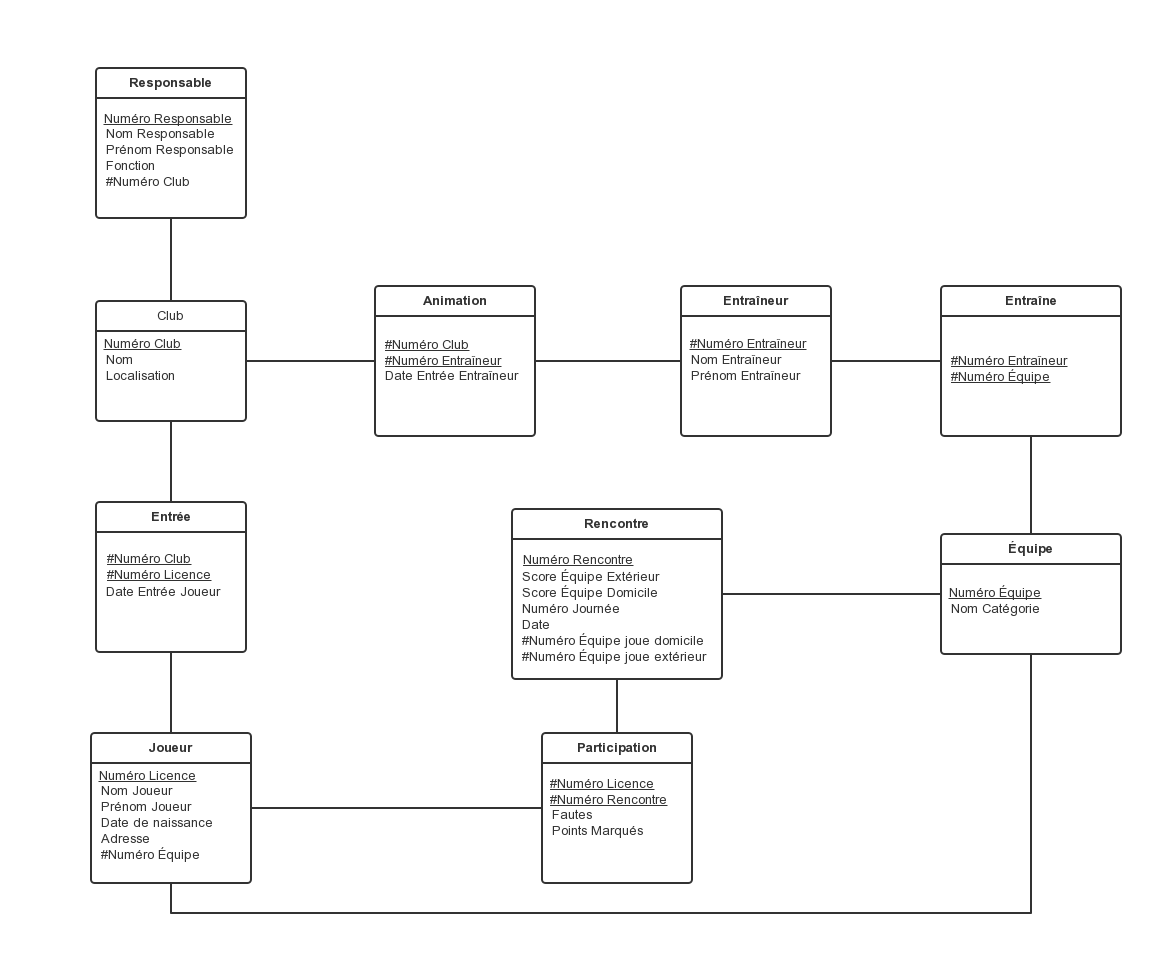
\includegraphics[scale=0.4]{ModeleRela.png}
\caption{Modèle Relationnel\label{ModeleRela}}
\end{figure}

\begin{mld}
  \relat{Club} & (\prim{numéro\_club}, \attr{nom\_club}, \attr{localisation})\\
  \relat{Responsable} & (\prim{numéro\_responsable}, \attr{nom\_responsable}, \attr{prénom\_responsable}, \attr{fonction}, \foreign{numéro\_club})\\
  \relat{Entraîneur} & (\prim{numéro\_entraîneur}, \attr{nom\_entraîneur}, \attr{prénom\_entraîneur}, \foreign{numéro\_club}, \attr{date\_entrée\_entraîneur})\\
  \relat{Animation} & (\prim{\foreign{numéro\_club},~\foreign{numéro\_entraîneur}}, \attr{date\_entrée\_entraîneur})\\
  \relat{Entraîne} & (\prim{\foreign{numéro\_équipe}}, \prim{\foreign{numéro\_entraîneur}})\\
  \relat{Équipe} & (\prim{numéro\_équipe}, \attr{nom\_catégorie})\\
  \relat{Joueur} & (\prim{numéro\_licence}, \attr{adresse\_joueur}, \attr{nom\_joueur}, \attr{prénom\_joueur}, \attr{date\_naissance\_joueur}, \foreign{numéro\_équipe}, \foreign{numéro\_club}, \attr{date\_entrée\_joueur})\\
  \relat{Entrée} & (\prim{\foreign{numéro\_club}, \foreign{numéro\_joueur}}, \attr{date\_entrée\_joueur})\\
  \relat{Participation} & (\prim{\foreign{numéro\_licence}}, \prim{\foreign{numéro\_rencontre}}, \attr{points\_marqués}, \attr{fautes})\\
  \relat{Rencontre} & (\prim{numéro\_rencontre},~\attr{date\_rencontre}, \attr{score\_équipe\_domicile}, \attr{score\_équipe\_extérieur}, \foreign{numéro\_équipe.1}, \foreign{numéro\_équipe.2})\\
\end{mld}

\section{Implémentation}
Nous avons utilisé une base de données MySQL. Les requêtes sont disponibles dans des fichiers sql. Dans cette partie, nous présentons uniquement certaines des requêtes que nous avons réalisées.

\subsection{Requêtes de création/suppression}
Les requêtes de création des tables sont classiques. Nous allons détailler le fonctionnement de la création d'une table sur la table \textsf{CLUB}.\\

Nous vérifions d'abord qu'une table \textsf{CLUB} n'est pas déjà existante. Si une telle table existe, on la supprime:\\
\fbox{drop table if exists CLUB cascade;}\\

On crée ensuite la table correspondant à notre modèle relationnel, on spécifie quelle est la clef primaire, on ajoute la condition qu'elle ne peut pas être nulle et qu'elle s'incrémentera automatiquement en cas d'ajout de données à cette table:\\

\begin{lstlisting}[language=SQL, caption=Initialisation Club, frame=shadowbox]
CREATE TABLE club
(
numero_club     INT(11)  NOT NULL AUTO_INCREMENT,
nom_club  CHAR(20),
localisation  CHAR(20),
    CONSTRAINT PK_ACTEUR PRIMARY KEY (numero_club)
);
\end{lstlisting}
\vspace{0.5cm}

En ce qui concerne l'ajout de données, il fallait faire attention à l'ordre dans lequel les entités étaient créées en raison de la création de clefs étrangères dans certaines entités. Nous avons donc ajouté en premier les entités qui ne possédaient pas de clefs étrangères, puis celles qui possédaient une clef étrangère vers une des classes créées. Voici l'exemple d'ajout des clubs :\\

\begin{lstlisting}[language=SQL, caption= Ajout des equipes, frame=shadowbox]
INSERT INTO club VALUES ( 1 , "Lakers" , "Los Angeles" ) ;
INSERT INTO club VALUES ( 2 , "Heat" , "Miami" ) ;
INSERT INTO club VALUES ( 3 , "Bulls" , "Chicago" ) ;
INSERT INTO club VALUES ( 4 , "Spurs" , "San Antonio" ) ;
INSERT INTO club VALUES ( 5 , "Celtics" , "Boston" ) ;
COMMIT ;
\end{lstlisting}

\subsection{Requêtes de mise à jour}
Les instructions pour réaliser les requêtes de mise à jour sont très similaires à celles d'ajout, il suffit de spécifier les champs que l'on veut modifier et remplacer le mot clef \textit{insert} par le mot clef \textit{update}.\\

Voici un exemple de mise à jour sur la table club:
\begin{lstlisting}[language=SQL, caption=Modification de la localisation d'un club, frame=shadowbox]
UPDATE club
SET club.localisation = "New York"
WHERE club.numero_club = 1;
\end{lstlisting}

Il suffit alors de vérifier l'intégrité des données à l'aide de déclencheurs.

\subsection{Requêtes de consultation}
\subsubsection{Informations générales}
Dans cette partie, nous allons présenter certaines des requêtes de consultation qui fournissent des informations sur différents éléments d'un club ou des informations sur tous les clubs de la fédération.

Les requêtes les plus simples sont celles qui permettent d'obtenir des informations sur l'entité club.
Il suffit de saisir simplement :
\fbox{\textit{SELECT} * \textit{FROM} club}\\
On peut alors affiner la demande en spécifiant un numéro de club ou un nom de club ou une localisation.

On peut réaliser des requêtes similaires sur les entités rencontre, responsable, joueur, entraîneur pour obtenir des informations comme les noms et prénom des membres d'un club.\\
\fbox{\textit{SELECT} * {FROM} {joueur}} fournit ainsi la listes des noms, prénoms, addresse, dates de naissance de tous les joueurs de la fédération.
On peut affiner ces requêtes en spécifiant certains critères comme le numéro de club, une date de naissance, une date d'entrée dans un club, \textit{etc}\dots\\

Voici quelques exemples :

\begin{lstlisting}[language=SQL, caption=Liste des joueurs d'un club, frame=shadowbox]
SELECT joueur.*
FROM joueur, entree, club
WHERE club.numero_club = entree.numero_club
AND entree.numero_licence = joueur.numero_licence
\end{lstlisting}

\begin{lstlisting}[language=SQL, caption=Liste des joueurs d'un club inscrits avant la «date voulue», frame=shadowbox]
SELECT joueur.*
FROM joueur, entree, club
WHERE club.numero_club = entree.numero_club
AND entree.numero_licence = joueur.numero_licence
AND entree.date_entree_joueur = "date_voulue"
\end{lstlisting}

\subsubsection{Statistiques}
Les requêtes fournissant les statistiques ont été les plus compliquées à réaliser. Elles font généralement intervenir plusieurs tables intermédiaires. La difficulté principale était de relier la table rencontre avec les autres entités dont nous voulions extraire des informations.
Parfois plus de quatre tables de notre base de données sont utilisées pour constituer la requête de statistique désiré. On les agence grâce à l'imbrication consécutive de select from(...)\\
La requête la plus globale est celle du classement des équipes intégrant le goalaverage de chacune d'entre-elles, pouvant les départager en cas d'égalité au nombre de points. Le système retenu est le suivant : 3 points en cas de victoire, 1 point en cas de match nul, 0 points en cas de défaite.

Pour des raisons de place, nous n'intégrerons pas dans ce rapport la requête de classement général des équipes d'une catégorie. Les exemples 1 et 2 sont des requêtes "passerelles" ayant permis de construire ce classement.
\\
\begin{itemize}
\item \textit{Exemple 1} : la requête permettant de connaitre le nombre de victoire à domicile de chaque équipe pour la catégorie senior, depuis le début de la saison. La catégorie est modifiable par l"utilisateur depuis l"interface de notre projet.
\begin{lstlisting}[language=SQL, caption=Victoire à domicile, frame=shadowbox]
SELECT vic_dom.numero_equipe, nombre_victoire_domicile,
nom_categorie
FROM (SELECT numero_equipe, count(rencontre.numero_rencontre)
as nombre_victoire_domicile
    FROM equipe
    LEFT JOIN rencontre
    ON rencontre.numero_equipe_joue_domicile = 
    	equipe.numero_equipe
    AND score_equipe_domicile > score_equipe_exterieur
    GROUP BY numero_equipe) AS vic_dom, equipe

WHERE equipe.nom_categorie = "senior"
AND vic_dom.numero_equipe = equipe.numero_equipe
ORDER BY nombre_victoire_domicile DESC
\end{lstlisting}

\item \textit{Exemple 2} : la requête permettant de connaitre le goalaverage de chaque équipe, soit la somme sur toute la saison de la différence entre le score de l'équipe et le score de l'équipe adverse à chaque rencontre. 
\begin{lstlisting}[language=SQL, caption=Goalaverage de chaque équipe, frame=shadowbox]
SELECT rtr_l.numero_equipe, 
IFNULL(diff_domicile,0)+IFNULL(diff_exterieur,0)
AS goalaverage_general
FROM (SELECT numero_equipe, 
SUM(score_equipe_domicile-score_equipe_exterieur)
AS diff_domicile
    FROM equipe
    LEFT JOIN rencontre
    ON rencontre.numero_equipe_joue_domicile
    	= equipe.numero_equipe
    GROUP BY numero_equipe) AS goal_l
LEFT JOIN    (SELECT numero_equipe, 
SUM(score_equipe_exterieur-score_equipe_domicile)
AS diff_exterieur
    FROM equipe
    LEFT JOIN rencontre
    ON rencontre.numero_equipe_joue_exterieur
    	= equipe.numero_equipe
    GROUP BY numero_equipe) goal_r
ON goal_l.numero_equipe = goal_r.numero_equipe
ORDER BY goalaverage_general DESC
\end{lstlisting}
Cette requête se construit selon la structure suivante :
\begin{enumerate}
\item Création de la table de goalaverage exterieur
\item Création de la table de goalaverage domicile
\item selection pour chaque équipe de leur goalaverage général (somme des colonnes diff\_exterieur et diff\_domicile de ces deux tables)
\end{enumerate}
\item \textit{Exemple 3} : en dernier exemple des requêtes de statistiques, la requête présentant les meilleurs joueurs d'une catégorie pour une journée, classés en fonction de leur points marqués et de leurs nombres de fautes commises. La catégorie et la journée sont choisis par l'utilisateur, ici égales respectivement à "junior" et 1.

\begin{lstlisting}[language=SQL, caption=Goalaverage de chaque équipe, frame=shadowbox]
SELECT DISTINCT nom_joueur, prenom_joueur,
participation.numero_licence, points, fautes
       FROM participation, joueur, rencontre, equipe
               WHERE joueur.numero_licence
               		= participation.numero_licence
        AND rencontre.numero_rencontre 
        	= participation.numero_rencontre
        AND (joueur.numero_equipe = numero_equipe_joue_domicile
        	or
            joueur.numero_equipe = numero_equipe_joue_exterieur)
        AND (equipe.numero_equipe = numero_equipe_joue_domicile 
        	or
             equipe.numero_equipe = numero_equipe_joue_exterieur)
        AND equipe.nom_categorie = "junior"
        AND numero_journee = 1
GROUP BY nom_joueur
ORDER BY points DESC, fautes ASC
\end{lstlisting}
\end{itemize}
 
\section{Interface}
L'interface fait intervenir le language PHP. Nous avons pris un soin particulier à avoir une organisation structurée du code (suivant autant que possible un pattern MVC), respectieuse à un niveau correct des principes élémentaires d'une application web (par effectuer une redirection après avoir soumis un formulaire), en mettant en pratique certains principes enseignés dans le module Web/XML.

\subsection{Installation}
Pour l'installation, il faut vérifier en premier lieu que l'extension \texttt{pdo\_mysql} est activée, et qu'une base de données MySQL est disponible.

Les identifiants de la base de données doivent être renseignés dans le fichier \texttt{app/config.php}.

Un bouton est alors disponible sur la page d'accueil pour créer les différentes tables ainsi que charger les fixtures.

Par ailleurs, une version mirroir est disponible à l'adresse \href{http://sgbd.silverwyrda.org}.

\subsection{Organisation du code}
Le code est partagé entre trois répertoires principaux: le premier est \texttt{src} contenant les sources, le second est \texttt{app} contenant la configuration de l'application, et enfin \texttt{web} contenant les contrôleurs (on se base sur le routage induit par l'arborescence des fichiers).

L'arborescence des fichiers sources est la suivante:
\begin{enumerate}
\item \texttt{models} contient les modèles des différentes entités d'une part, et les \emph{repository} associés à chacune des entités permettant de regrouper certaines requêtes d'autre part,
\item \texttt{templates} contenant des fichiers .php équivalents à des templates, au sens où on ne fait que de l'affichage,
\item \texttt{modules} contenant quelques utilitaires, notamment pour partager la connexion à la base de données ainsi qu'une fonction permettant de faire le rendu d'un template.
\end{enumerate}

\subsection{Organisation du site}
L'interface se concentre en premier sur le club et implémente depuis cette entité des accès aux différentes relations, en cascade. Des listes sont également disponibles pour chaque entité principale permettant d'accéder à des fonctions de suppression et d'édition lorsqu'elles sont implémentées. L'accent a été mis sur la simplicité de l'interface en évitant d'agréger beaucoup de données sur une seule page (en pratique uniquement les relations directes sont reflétées).

Concernant l'aspect visuel, nous avons utilisé le framework \emph{Foundation} qui a la particularité de forcer une bonne structure du code HTML sans pour autant dénaturer sa nature première de transmission de données, et non de mise en forme de celle-ci. Ceci permet enfin d'avoir une interface propre sans perdre de temps à travailler sur le design.

\section{Conclusion}
Ce projet a été l'occasion de développer et d'approfondir les connaissances acquises en TD, à la fois en ce qui concerne les diagrammes entité-association que les diagrammes relationnels ou la maîtrise de MySQL. En premier lieu, il a fallu bien définir les limites du sujet afin d'obtenir un modèle cohérent de fédération de basket, chaque table devant respecter les 3 formes normales. Ensuite, la partie codage a été composée de l'ajout de la base suivant le fonctionnement du modèle créé, l'ajout de données suffisantes dans la base afin de satisfaire un certain nombre de requêtes, et l'ajout des requêtes demandées dans le sujet. Enfin, la partie interface réalisée en PHP consent à apporter un confort à l'utilisateur que ce soit pour l'ajout de données, la consultation des tables ou de requêtes de statistiques, notamment le classement général des équipes.

\end{document}